% ----------------------------------------------------------------------- %
% Arquivo: cap2.tex
% ----------------------------------------------------------------------- %

\chapter{Alguns conceitos}
\label{c_cap2}

É a parte principal do texto. Apresenta o assunto, fundamentação teórica, metodologia (materiais e métodos), os resultados e as respectivas discussões traçando relações com os trabalhos analisados na revisão de literatura.

\section{Revisão de literatura}\label{s_c2_revisao}

É uma análise comentada sobre o que já foi publicado sobre o assunto da pesquisa, buscando mostrar os pontos de vista convergentes e divergentes entre os autores. Traça-se um quadro teórico e elabora-se a estruturação conceitual que subsidiará o desenvolvimento da pesquisa. A revisão de literatura permitirá um mapeamento de quem já escreveu e o que já foi escrito sobre o assunto ou o problema de pesquisa.







\section{A inclusão de figuras}
\label{s_c2_figuras}

As figuras são bastante úteis para ajudar expressar o funcionamento, modelo, etc. de alguma parte de seu trabalho. No Linux existem diversas aplicações para a criação de figuras, sendo o Xfig\footnote{\url{http://www.xfig.org}} uma ótima opção para a criação de figuras com alta qualidade, apesar de sua interface não ser muito amigável. Muitos utilizam outras aplicações com interfaces mais amigáveis e que ainda assim geram figuras com uma qualidade razoável como o \textit{Inkscape}, \textit{DIA}, \textit{OpenOffice Draw}, \textit{Kivio}, etc.

A inclusão de figuras no texto necessita que algumas regras sejam atendidas. São essas:

\begin{itemize}
	\item As figuras deverão ser de alta qualidade;
	\begin{itemize}
		\item Evite colocar fotos e outras figuras complexas;
		\item Opte por figuras simples e que realmente expressem algo, mesmo quando impressas em preto e branco;
	\end{itemize}
	\item Em \LaTeX~as figuras deverão estar nos formatos: \texttt{PDF}, \texttt{JPG} ou \texttt{PNG};
	\item Toda figura deverá possuir uma legenda;
	\item Toda figura deverá ser referenciada em alguma parte do texto.
\end{itemize}

A \autoref{f_c2_disco} foi inserida no texto para mostrar como fazer tal inserção em \LaTeX. Vale lembrar que toda figura inserida deverá ser, em algum momento, referenciada no texto. 

\begin{figure}[!htpb]
	\centering
	\caption{Disquete}\label{f_c2_disco}
	%\includegraphics[width=5cm]{03.2.1_fig/disco}
    \includegraphics[width=5cm]{03-elementos/03.2_textual/03.2.1_fig/disco.pdf}
\end{figure}

O objetivo deste documento é de mostrar como preparar uma monografia para o curso de Engenharia de Telecomunicações. No ~\autoref{c_cap3} é apresentado uma forma para fazer citações de outros trabalhos. O capítulo ainda apresenta uma forma para incluir tabelas no documento. O ~\autoref{c_conclusoes} apresenta as conclusões deste trabalho além de apresentar os trabalhos futuros.

\subsection{Mascotes}
\label{s_c2_mascotes}

Essa é uma subseção da \autoref{s_c2_figuras} do \autoref{c_cap2}. 

\begin{figure}[ht]
	\centering
	\caption{O mascote do~\LaTeX~em diferentes poses}\label{f_c2_mascotes}
	\subcaptionbox{O mascote estudando\label{f_c2_masco1}}
		{
\includegraphics[width=.4\textwidth]{03-elementos/03.2_textual/03.2.1_fig/lion.pdf}}
	\subcaptionbox{O mascote ensinando\label{f_c2_masco2}}
		{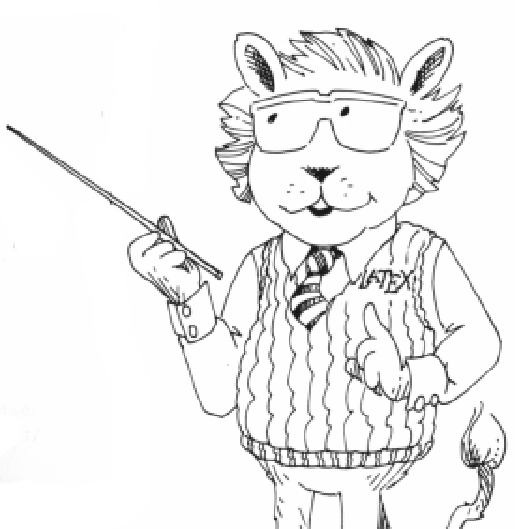
\includegraphics[width=.4\textwidth]{03-elementos/03.2_textual/03.2.1_fig/latex_lion.pdf}}
\end{figure}


A \autoref{f_c2_mascotes} ilustra uma forma de incluir duas figuras, lado a lado, usando o pacote \texttt{subcaption}. A \autoref{f_c2_masco1} ilustra o mascote do \LaTeX~estudando. Já na \autoref{f_c2_masco2} o mascote aparece apresentando algum assunto. 


\section{Como apresentar equações}
\label{s_c2_equacoes}

O \LaTeX é um pacote feito para a preparação de textos impressos de alta qualidade, especialmente
para textos matemáticos. Ele foi desenvolvido por Leslie Lamport a partir do programa
\TeX~criado por Donald Knuth.

Fórmulas matemáticas são produzidas digitando no arquivo fonte texto descrevendo-as. Isto
significa que o \LaTeX~deve ser informado que o texto que vem a seguir é uma fórmula e também
quando ela termina e o texto normal recomeça. As fórmulas podem ocorrer em uma linha de
texto como $ax^2 + bx + c = 0$, ou destacada do texto principal como na \autoref{e_c2_eq1}.

\begin{equation}
 x=\frac{-b\pm\sqrt{b^2-4ac}}{2a}
\label{e_c2_eq1}
\end{equation}

\section{Incluindo trechos de códigos}

Em alguns casos é desejado incluir trechos de códigos no documento. O \LaTeX oferece inúmeras maneiras para isto e o pacote \textbf{listings} é conhecido por apresentar um dos melhores resultados. A \autoref{l_olamundo} apresenta o código em \textit{shell script} para o complexo problema do ``Olá mundo!''. A \autoref{l_matlab} apresenta um trecho de código em MatLab.

%parâmetros: linguagem (shell, java, matlab, python, c, php), label, caption, arquivo

\includecode[shell]{l_olamundo}{Olá mundo em shell script}{03-elementos/03.2_textual/03.2.0_codes/ola.sh}

\includecode[matlab]{l_matlab}{Um pequeno código em MatLab}{03-elementos/03.2_textual/03.2.0_codes/matlab.m}

% ---
\section{Divisões do documento: seção}\label{sec-divisoes}
% ---

Esta seção testa o uso de divisões de documentos. Esta é a
\autoref{sec-divisoes}. Veja a \autoref{sec-divisoes-subsection}.

\subsection{Divisões do documento: subseção}\label{sec-divisoes-subsection}

Isto é uma subseção. Veja a \autoref{sec-divisoes-subsubsection}, que é uma
\texttt{subsubsection} do \LaTeX, mas é impressa chamada de ``subseção'' porque
no Português não temos a palavra ``subsubseção''.

\subsubsection{Divisões do documento: subsubseção}
\label{sec-divisoes-subsubsection}

Isto é uma subsubseção.

\subsubsection{Divisões do documento: subsubseção}

Isto é outra subsubseção.

\subsection{Divisões do documento: subseção}\label{sec-exemplo-subsec}

Isto é uma subseção.

\subsubsection{Divisões do documento: subsubseção}

Isto é mais uma subsubseção da \autoref{sec-exemplo-subsec}.


\subsubsubsection{Esta é uma subseção de quinto
nível}\label{sec-exemplo-subsubsubsection}

Esta é uma seção de quinto nível. Ela é produzida com o seguinte comando:

\begin{verbatim}
\subsubsubsection{Esta é uma subseção de quinto nível}
\label{sec-exemplo-subsubsubsection}
\end{verbatim}

\subsubsubsection{Esta é outra subseção de quinto nível}\label{sec-exemplo-subsubsubsection-outro}

Esta é outra seção de quinto nível.


\paragraph{Este é um parágrafo numerado}\label{sec-exemplo-paragrafo}

Este é um exemplo de parágrafo nomeado. Ele é produzida com o comando de
parágrafo:

\begin{verbatim}
\paragraph{Este é um parágrafo nomeado}
\label{sec-exemplo-paragrafo}
\end{verbatim}

A numeração entre parágrafos numeradaos e subsubsubseções são contínuas.

\paragraph{Esta é outro parágrafo numerado}\label{sec-exemplo-paragrafo-outro}

Esta é outro parágrafo nomeado.

% ---
\section{Este é um exemplo de nome de seção longo. Ele deve estar
alinhado à esquerda e a segunda e demais linhas devem iniciar logo abaixo da
primeira palavra da primeira linha}
% ---

Isso atende à norma \citeonline[seções de 5.2.2 a 5.2.4]{NBR14724:2011} 
 e \citeonline[seções de 3.1 a 3.8]{NBR6024:2012}.


\section{Usando siglas e abreviaturas}

Algumas vezes nos deparamos com textos cheios de siglas. O \LaTeX provê ferramentas para gerar glossário, lista de acrônimos, etc. Neste parágrafo é feito uso de comandos definidos no pacote \textit{acronym} e a listagem de acrônimos fica dentro do arquivo \texttt{abreviaturas.tex}.

O protocolo \ac{TLS} deve ser empregado sempre que se deseja garantir a integridade e a confidencialidade das mensagens trocadas pela rede. O \ac{TLS} é hoje utilizado por diversas aplicações. Como faz tempo que eu não falo do \acf{TLS} eu chamo o nome completo mais a sigla, ajudando o meu leitor a lembrar da sigla \ac{TLS}. Existe a \ac{AC} que é bem importante. Este documento segue as normas da \ac{ABNT} e para isso faz uso do pacote \ac{abnTeX}.